\documentclass{endm}
\usepackage{endmmacro}
\usepackage{graphicx}
\usepackage{amsmath}
\usepackage{cases}
\usepackage{caption}
\usepackage[brazilian,english]{babel}
\usepackage[utf8]{inputenc}
\usepackage[T1]{fontenc}

% The following is enclosed to allow easy detection of differences in
% ascii coding.
% Upper-case    A B C D E F G H I J K L M N O P Q R S T U V W X Y Z
% Lower-case    a b c d e f g h i j k l m n o p q r s t u v w x y z
% Digits        0 1 2 3 4 5 6 7 8 9
% Exclamation   !           Double quote "          Hash (number) #
% Dollar        $           Percent      %          Ampersand     &
% Acute accent  '           Left paren   (          Right paren   )
% Asterisk      *           Plus         +          Comma         ,
% Minus         -           Point        .          Solidus       /
% Colon         :           Semicolon    ;          Less than     <
% Equals        =           Greater than >          Question mark ?
% At            @           Left bracket [          Backslash     \
% Right bracket ]           Circumflex   ^          Underscore    _
% Grave accent  `           Left brace   {          Vertical bar  |
% Right brace   }           Tilde        ~

\newcommand{\Nat}{{\mathbb N}}
\newcommand{\Real}{{\mathbb R}}
\def\lastname{Brito}

\begin{document}  

% DO NOT REMOVE: Creates space for Elsevier logo, ScienceDirect logo
% and ENDM logo
\begin{verbatim}\end{verbatim}\vspace{2.5cm}

\begin{frontmatter}

\title{On the Fast Creation of Conflict Graphs for Integer Programs: A Computational Study}

\author{Samuel Souza Brito \and Haroldo Gambini Santos\thanksref{mailSamuelHaroldo}}
 
\address{Departamento de Computação\\ Universidade Federal de Ouro Preto - UFOP\\ Ouro Preto, Brazil}
\author{Marcus V. S. Poggi de Aragão\thanksref{mailPoggi}}
\address{Departamento de Informática\\ Pontifícia Universidade Católica do Rio de Janeiro - PUC-RIO\\ Rio de Janeiro, Brazil}
\thanks[mailSamuelHaroldo]{Email: {\texttt{\normalshape {samuelsouza,haroldo}@iceb.ufop.br}}} 
\thanks[mailPoggi]{Email: {\texttt{\normalshape poggi@inf.puc-rio.br}}}  

\begin{abstract}
Conflict graphs are employed in modern Integer Programming to store relationships between variables. This information is crucial for an effective pre-processing and cut generation. CGs can be dynamically built inside branch-and-bound algorithms while analyzing the impact of the last fixations performed, but the earlier the CG is populated the faster strong inequalities and implications can be generated. On this work we present techniques which allow the fast creation of densely populated CGs at the root node. The impact of the availability of these large GCs for cut generation is evaluated by the inclusion of these techniques in the state-of-the-art open source integer programming solver COIN-OR CBC and its use in a cutting plane algorithm.
\end{abstract}

\begin{keyword}
conflict graphs, integer programming, clique cuts, set packing polytope
\end{keyword}

\end{frontmatter}


\section{Introduction}\label{intro}

In this work we present an approach for the creation of conflict graphs for Integer Programming (IP) problems. A Conflict Graph (CG) represents logical relations between binary variables. This kind of graph has a vertex for each binary variable and its complement. An edge between two vertices indicates that variables involved cannot be set to some specific value at the same time without violating one or more constraints.

CGs are typically constructed using probing techniques \cite{Borndorfer1998} based on constraints analysis. The probing technique consists in analyzing logical implications generated by fixing binary variables.  Building a graph by looking for pairwise of conflicts may be computationally prohibitive when the input problem is large. Thus, the computational efficiency of this technique depends on the complexity of the constraint exploration, causing a trade off between efficiency and effectivity. 

On this work we propose techniques to speed up the creation of dense conflict graphs at the root node, so that large CGs can be available at the start of the search process for the generation of strong inequalities. For ease of understanding of our approach we consider only pure Binary Programs (PB). Despite this, it can be applied to any Integer Program containing binary variables. 

The rest of the paper is organized as follows. In Section \ref{seccgraph}, we formally explain our approach to build conflict graphs as well our strategy to speedup the detection of logical implications. In Section \ref{cut}, we present the clique cut separation routine, including a clique extension step. In Section \ref{experiments}, the computational experiments with instances of MIPLIB 2010 \cite{miplib}, International Nurse Rostering Competition \cite{haspeslagh} and Telebus problem \cite{Borndorfer1998} are presented and analyzed. Finally, in Section \ref{conclusions}, we conclude and give future directions about this work.

\section{Conflict Graphs in Integer Programming}\label{seccgraph}

A conflict graph represents logical relations between binary variables. For two binary variables, we may discover four possible logical relations, using the notation of \cite{atamturk}:


\begin{align}
x = 1 \Rightarrow y = 1 & \quad \Longleftrightarrow \quad x + (1 - y) & \leq \ 1\\
x = 1 \Rightarrow y = 0 & \quad \Longleftrightarrow \quad x + y & \leq \ 1 \\
x = 0 \Rightarrow y = 1 & \quad \Longleftrightarrow \quad (1 - x) + (1 - y) & \leq \ 1 \\
x = 0 \Rightarrow y = 0 & \quad \Longleftrightarrow \quad (1 - x) + y & \leq \ 1
\end{align}

Given an Integer Programming (IP), a conflict graph can be constructed using probing techniques based on feasibility considerations\cite{atamturk,achterberg,sandholm}, checking the impact fo fixing pairs of variables to different combinations of values. First, consider that each constraint $i \in \{1,\ldots,m\}$ can be written as:

\begin{equation}
 \sum_{j \in N} a_{ij}x_{j} \leq b_{i} 
\end{equation}

\noindent where $N$ is the index set of binary variables $x$, $a_{ij}$ is the coefficient for variable $x_{j}$ at constraint $i$ and $b_{i}$ is the right-hand side of constraint $i$. Suppose we are analyzing two particular variables $x_{\hat{j}}$ and $x_{\hat{k}}$ with respect to constraint $i$. Consider that these variables are assigned with values $u$ and $v$, respectively. Let:

\begin{equation}\label{li}
L_{i}^{x_{\hat{j}} = u,\, x_{\hat{k}} = v}=\sum_{j\in N_{i}^{-} \setminus \{\hat{j}, \hat{k}\}}a_{ij}+a_{i\hat{j}}u+a_{i\hat{k}}v 
\end{equation}

\noindent where $N_{i}^{-} = \{j \in N : a_{ij} < 0\}$. In this case, $L_{i}^{x_{\hat{j}} = u,\, x_{\hat{k}} = v}$ is a lower bound for the value on the left-hand side  of the constraint $i$, considering the assignments $x_{\hat{j}} = u$ and $x_{\hat{k}} = v$. If $L_{i}^{x_{\hat{j}} = u,\, x_{\hat{k}} = v} > b_{i}$, there is a conflict between the assignments of $x_{\hat{j}}$ and $x_{\hat{k}}$. 

Performing these steps for each combination of values of two binary variables, considering each pair of variables in each constraint, leads to the creation of a conflict graph in $O(m \times n^2)$. For problems with many variables and constraints this technique may be expensive computationally (See Experiments section). Nevertheless, for some constraint types a large number of conflicts can be quickly discovered. This is the case of the Generalized Upper Bound constraints ($\sum_{j\in N}x_j \leq 1$). As discussed in \cite{atamturk}, even handling explicitly conflict graphs induced by these constraints requires special data structures such that in the previous decade most solvers could not use all information which could be inferred just from GUB constraints. The following subsection will describe additional cases where cliques in individual constraints can be quickly detected (i.e., faster than $O(n^2)$). The following notation will be used: $\tilde{a}_{ik}$ is the $k$-th smallest coefficient in constraint $i$ and $\acute{a}_{ik}$ indicates its index. Constants $n_i$ and $S_i^-$ denote the number of non-zero variables and the sum of all negative coefficients of constraint $i$, respectively. In the next subsection fast clique detection will be discussed for additional constraint structures.


\subsection{Fast detection of cliques in less structured constraints}

We describe two simple cases where large cliques of conflicting variables can be detected just by traversing constraints with  coefficients of variables sorted in non-decreasing order. Thus, conflicts in these constraints are discovered in $O( n \log n)$. At first, consider that at a given position $k$ the summation of negative coefficients excluding the pair of variables at positions $k$ and $k+1$ is: 

\begin{equation}\label{di}
D_{i}^{x_{\acute{a}_{ik}}, x_{\acute{a}_{ik+1}}} = S_i^- - min(0, \tilde{a}_{ik}) - min(0, \tilde{a}_{ik+1})
\end{equation}

\noindent Thus, the lower bound for the LHS of constraint $i$ when variables with the $k-th$ and $(k+1)-the$ smallest coefficients are fixed at one is:

\begin{equation}
LHS_{i}^{x_{\acute{a}_{ik}} = 1, x_{\acute{a}_{ik+1}} = 1} = D_{i}^{x_{\acute{a}_{ik}}, x_{\acute{a}_{ik+1}}} + \tilde{a}_{ik} + \tilde{a}_{ik+1}
\end{equation}

Since $LHS_{i}^{x_{\acute{a}_{ik}} = 1, x_{\acute{a}_{ik+1}} = 1}$ is monotonically non-decreasing as $k$ increases, if $LHS_{i}^{x_{\acute{a}_{ik}} = 1, x_{\acute{a}_{ik+1}} = 1} > b_{i}$, then there is a clique involving the activation of all variables from position $k$ until position $n_i$. Moreover, we can discard the existence of such cliques by checking if $LHS_{i}^{x_{\acute{a}_{in_i-1}} = 1, x_{\acute{a}_{in_i}} = 1} \leq b_i$. Analogously, cliques involving complimentary variables from positions $n_i$ until $k$ can be obtained or discarded checking if the limit incurred from positions $k$ and $k-1$  $LHS_{i}^{x_{\acute{a}_{ik}} = 0, x_{\acute{a}_{ik-1}} = 0} = D_{i}^{x_{\acute{a}_{ik}}, x_{\acute{a}_{ik-1}}} $ surpasses the upper bound $b_i$.

For variables which are not involved in these easy to compute cliques a pairwise analysis is performed for each constraint. 



\begin{figure}[h]
\begin{minipage}[b]{.5\textwidth}
\[
\mathcal{P} = \left\{
\begin{array}{lr}
x_1+x_2+x_3 & \geq 2 \\
-2x_{1}+3x_{2}+4x_{3}+5x_{4} & \leq 4 \\
x_{1},\ldots,x_{4}\in\{0,1\}
\end{array}
\right.
\]

\end{minipage}
\begin{minipage}{.5\textwidth}
	\centering
	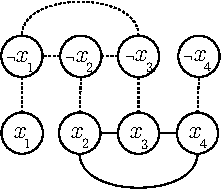
\includegraphics[width=3.2cm]{cGraph.pdf}
\end{minipage}
\caption{A binary program and its conflict graph}\label{graph}
\end{figure}


As an illustrative example, Figure \ref{graph} shows the conflict graph for a binary program $\mathcal{P}$, where $\neg x_i$ represents the complement (or deactivation) of variable $x_i$.  For the first constraint, analyzed as $(-x1-x2-x3\leq-2)$, we have a clique involving all complimentary variables since $LHS_1^{x_1=0,\, x_2=0}=-1$ which is greater than -2. For the second constraint $LHS_2^{x_2=1,\, x_3=1}=5$ indicates a clique from $x_2,x_3,x_4$, since these coefficients are in non decreasing order.

\section{Cutting Planes}\label{cut}

Linear programming relaxations can be significantly strengthened by the inclusion of inequalities derived from the set packing polytope (SPP) \cite {Padberg1973}. The most common classes of cuts for SPP are the clique cuts and the odd-hole cuts. A clique inequality for a set $C$ of conflicting variables has the form $\sum_{j\in C}x_{j} \leq 1$ and an odd-hole inequality with conflicting variables $C$ can be defined as: $\sum_{j\in C}x_{j} \leq \lfloor \frac{|C|}{2}\rfloor$. It is well known that in practice clique cuts are by far the most important ones \cite{Borndorfer1998}. The impact of these cuts has been explored for some hard timetabling problems \cite{Avella2005,Marecek2012}. Considering generic clique separation routines, the most common ones are the star clique and the row clique method \cite{Eso1999a,Hoffman1993,Borndorfer1998}. These are fast separation routines which are used in the current version of the COIN-OR Cut Generation Library.  

Our algorithm proposal considers aggressive clique separation: instead of searching for \emph{the} most violated clique inequality we search for \emph{all} violated clique inequalities. Some previous results indicate that this is the best strategy. In \cite{Marecek2012}, for example, although authors used a branch-and-bound code to search for the most violated clique, computational results motivated the inclusion of non-optimally violated cuts found during the search. This result is consistent with reports of application of other cuts applied to different models, such as {C}hv\`{a}tal-Gomory cuts \cite{Fischetti2007}. The option for inserting a large number of violated inequalities at once is also responsible for reviving the gomory cuts importance \cite {Cornuejols2007}.

Our proposed clique separation routine has two main components:  \begin{enumerate} \item a module to separate all violated cliques in the conflict subgraph induced by the fractional variables; \item a lifting module which extends generated cliques considering the original conflict graph. \end{enumerate}  The clique separation module was implemented using an improved version of the Bron-Kerbosch algorithm \cite{Bron1973}. This version implements an optimized pivoting rule \cite{Brito2011} to speed up the discovery of maximal cliques with large weight. This rule assigns the highest priority for visiting first nodes with large modified degree (summation of node degree and of its neighbors) and weight. Although this algorithm has an exponential worst case performance, the heuristic pivot rules  make the algorithm suitable not only for running in the enumeration context but also for executing with restricted times, since larger violated cliques tend to be discovered first. Nevertheless, our experiments showed that all violated inequalities for all instances can be enumerated in a fraction of a second using our implementation. It is also important to remark that even if a subset of cliques is inserted, the optimal solution would not be missed, branching would take care of the rest.  The importance of lifting clique inequalities can be explained with the conflict graph in Figure \ref{figClique}. Nodes inside the gray area indicate variables with non-zero values in the fractional solution. In this solution, only nodes $x_{2},\ldots,x_{4}$ could contribute to define a maximally violated clique inequality. Nevertheless, subsequent linear programming relaxations could include three different violated $k_{3}$\footnote{a clique with three nodes} cliques by alternating the inactive variable. If the $k_{4}$ clique inequality were inserted during the separation of the first fractional solution, additional re-optimizations of the linear program could be saved. Furthermore, a less dense constraint matrix may be obtained with the insertion of these dominant constraints first.

\begin{figure}
\begin{center}
	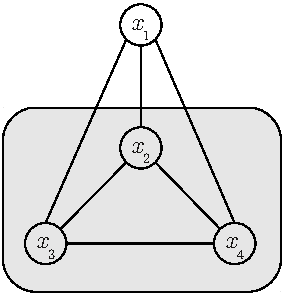
\includegraphics[width=0.3\textwidth]{clique.pdf}
	\caption{Example of a $k_{3}$ which could be lifted to a $k_{4}$ } \label{figClique}
\end{center}
\end{figure}

It is well known that the separation of odd-holes contributes only marginally for lower bound improvement \cite{Borndorfer1998,Mendez-Diaz2008}. Nevertheless, its inclusion in the branch-and-cut procedure is cheap, since these inequalities can be separated in polynomial time using shortest path algorithms \cite{Grotschel1993}. Odd hole inequalities can be strengthened by the inclusion of a wheel center, such as variable $x_{6}$ in the conflict graph presented in Figure \ref{figOH}. In fact, for an odd hole with variables $C$ and $W$ being the set of candidates to be included as wheel centers of $C$, the following inequality is valid:

\begin{equation}
	\sum_{j \in W} \lfloor \frac{|C|}{2} \rfloor x_{j} + \sum_{j \in C} x_{j} \leq \lfloor \frac{|C|}{2} \rfloor
\end{equation}

\begin{figure}
\begin{center}
	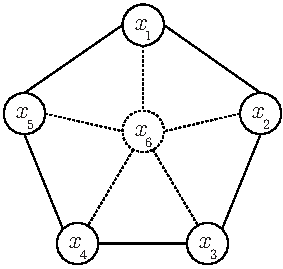
\includegraphics[width=0.3\textwidth]{oddHole.pdf}
	\caption{Example of an odd hole and its possible extension to a wheel} \label{figOH}
\end{center}
\end{figure}


\section{Experimental Results}\label{experiments}

Our code was written in C/C++ using the open source COIN-OR libraries. These libraries allowed us to integrate our routines with the COIN-OR MIP solvers \cite{Forrest2005,Linderoth2005,Ralphs2005} and also communicate with commercial solvers through the Open Solver Interface (OSI) \cite{Saltzman2004}. The code was compiled on GCC/G++ version 4.8.3. We ran all the experiments on Intel Core i7 3.60GHz computers with 32GB of RAM running Linux openSUSE 13.2 64 bits.

The dataset used consists of problems with varying characteristics. The first set of instances is the benchmark set of MIPLIB 2010 \cite{miplib}, containing 87 instances. Since its introduction in 1992, the MIPLIB became a standard library of tests used to compare the performance of integer programming solvers. It contains a collection of real problems, most of them based on industrial applications. The second set of instances is the same used during the International Nurse Rostering Competition \cite{haspeslagh}, containing 69 instances. This competition aimed to encourage research in the field of scheduling and establish a benchmark problem that was widely accepted by the scheduling community. In addition, it allowed researchers could compare their results accurately and fairly. Finally, the last problem set is formed by instances of Telebus problem \cite{Borndorfer1998}, containing 56 instances. Telebus problem consists of a vehicle scheduling problem, whose objective is to choose the right fleet and appropriate vehicle rotations to service all orders. Such problems can be attacked with a set partitioning approach of combinatorial optimization.


\section{Conclusions and Future Work}\label{conclusions}

\bibliographystyle{endm}
\bibliography{references}

\end{document}
